To estimate experimentally the relative rate of non-equilibrium
processes one has to know both, the total production cross section
of given IMF and the cross section for its non-equilibrium emission.
The total production cross section may be in principle obtained by a
straightforward integration over energy and scattering angle of the
experimental differential cross sections $d\sigma/d\Omega dE$,
however the production cross section of given IMF due to a
non-equilibrium process cannot be extracted from the experiment
without additional model assumptions.  The most promising method for
this purpose seems to be substraction of the \emph{equilibrium}
emission cross section of given IMF  from its total production cross
section. Such a method should give value of the non-equilibrium
production cross section as reliable as that of the equilibrium
emission processes.  %Since the models which describe  emission of
%fragments from excited, equilibrated nuclei have been developed and
%improved since a very long time it is reasonable to expect that
%their predictive power is much better than that of other reaction
%mechanisms.
\section{IMF production cross sections in p + Ag reaction at 480 MeV}


It was demonstrated in the recent publications concerning predictive
power of various reaction models used for the description of
isotopic production cross sections in p+$^{136}$Xe collisions at 1
GeV/nucleon \cite{singh2018predictive} and at 0.5 GeV/nucleon \cite{sharma2017ranking}
as well as for the analysis of differential cross sections of
spallation reactions in p+Ag collisions at 0.48 GeV/nucleon
\cite{sharma2016ranking} that the description of data by GEMINI model\cite{CHARITY1988,Charity2010}[ref AIEEE] coupled to INCL4.6
\cite{boudard2013new} is superior in respect to those obtained with
three other, popular models of the second stage of the reaction,
namely ABLA07 \cite{kelic2009abla07}, SMM \cite{SMMBondorf1995} and GEM2 \cite{FURIHATA2000,Furihata2002}. Moreover, it was found that among
the above listed models only GEMINI does not produce cross sections
which exceed magnitude of the experimental data leaving a room for
another reaction mechanism contributing incoherently to the
reactions studied \cite{sharma2016ranking}.




The following procedure has been used for the estimation of the
equilibrium processes contribution to the production of the
intermediate mass fragments. It was assumed that the collision of
proton impinging on to the silver target proceeds as the two step
process. The INCL++ model (version 5.3) \cite{Mancusi2014} of the
intranuclear cascade has been used for description of the first,
fast stage of the collisions.
%
%The first, fast stage of the reaction consists in intranuclear
%cascade of nucleon-nucleon and nucleon-pion collisions which at the
%end leaves the excited, residual nucleus in the thermodynamical
%equilibrium. Such a compound nucleus decays further by emission of
%nucleons, light charged particles (LCP) and intermediate mass
%fragments (IMF) eventually (for the heaviest atomic nuclei) it may
%be a subject of nuclear fission.
%
%In the present study the INCL++ model (version 5.3)
%\cite{Mancusi14A} of the intranuclear cascade has been used.
%
A possibility of the emission of complex light charged particles in
this stage of the process has been taken into account to assure
achieving a realistic mass, charge and excitation energy
distribution of the residual compound nuclei. However, the
coalescence of the nucleons escaping from the intranuclear cascade
with creation of intermediate mass fragments was not allowed because
of two reasons: (i) the INCL++ enables one to perform efficiently
such calculations only for the lightest IMF \cite{boudard2013new}  and,
(ii) it was found in the earlier study of these reactions
\cite{sharma2016ranking} that high energy spectra of IMF are significantly
overestimated by this model.  It is important to emphasize that the
above decision does not modify significantly the mass, charge and
energy distribution of the excited nuclei - the remnants of the
cascade since the cross sections for production of IMF are orders of
magnitude smaller than those for nucleons and complex LCP. The
second stage of the process, i.e., emission of particles from the
excited compound nuclei - residuals of the fast stage of the
reactions was described by GEMINI++ model \cite{GEMINI++}.  The
results of the above calculations were treated as a realistic
estimation for the total as well as for differential cross sections
of equilibrated emission of IMF.

To obtain the total production cross section, the GEMINI++ double
differential cross sections $d^2\sigma/dEd\Omega$ were supplied by
incoherently added isotropic emission from highly excited Maxwellian
source (or two sources) moving along the beam direction. The
parameters of the source, i.e., its velocity $\beta$, apparent
temperature T, the contribution to the total cross section $\sigma$
and the parameters responsible for the Coulomb barrier hindering the
emission of ejectiles from the source were fitted to reproduce
simultaneously the spectra of given ejectile at all scattering
angles. Details of the moving source model as well as the
interpretation of its parameters  can be found in the Appendix of
Ref.\cite{bubak2007non}.

Very good reproduction of most of the data was achieved using one
moving source contribution. %to represent non-equilibrium part of the
%cross sections.
This is illustrated by Fig. \ref{fig:18OGEMINIS2} in which
experimental (dots) and model (lines) energy spectra of $^{18}$O
particles are depicted at three scattering angles: 20$^{\circ}$,
90$^{\circ}$ and 160$^{\circ}$.  As can be seen, the equilibrium
emission evaluated according to GEMINI++ \cite{GEMINI++} coupled to
INCL++ \cite{Mancusi2014} model (solid, blue line) gives practically
isotropic contribution whereas the non-equilib\-rium emission
represented by single moving source (dashed, red line) dominates at
forward scattering angle but it is much smaller than equilibrium
cross sections at backward angles. The sum of both contributions
(solid, black line) satisfactorily well reproduces the data.

Only 10 lightest IMF among all 39 studied particles, \emph{i.e.},
$^{6,7}$Li, $^{7,9,10}$Be, $^{10,11,12}$B and $^{11,12}$C needed
application of two moving sources for the good reproduction of
energy spectra at all investigated scattering angles from
20$^{\circ}$ to 160$^{\circ}$.  An example of obtained quality of
the data reproduction is presented in Fig. \ref{fig:9BeGEMINIS2S3}
where the energy spectra of $^9$Be emitted at the same scattering
angles as in Fig. \ref{fig:18OGEMINIS2}, \emph{i.e.},  20$^{\circ}$,
90$^{\circ}$ and 160$^{\circ}$ are shown.  The equilibrium emission
contribution represented by solid, blue line is in this case
significantly smaller than the data for all scattering angles. For
forward scattering angle and small energies the slower of both
moving sources gives dominating contribution - shown as a dashed,
red line - whereas the contribution of faster of the moving sources
- depicted as a dotted, magenta line - reproduces the high energy
tail of the spectrum.  The situation is different for large
scattering angle where the slower moving source dominates again for
small energies but it gives comparable to the faster source
contribution to the cross section at high energies.  This is a
typical situation for all analyzed spectra for which introduction of
two moving sources was necessary.
%
%
%\begin{figure*}
\begin{figure}
  % Requires \usepackage{graphicx}
  \centering
  \resizebox{0.5\textwidth}{!}{%
  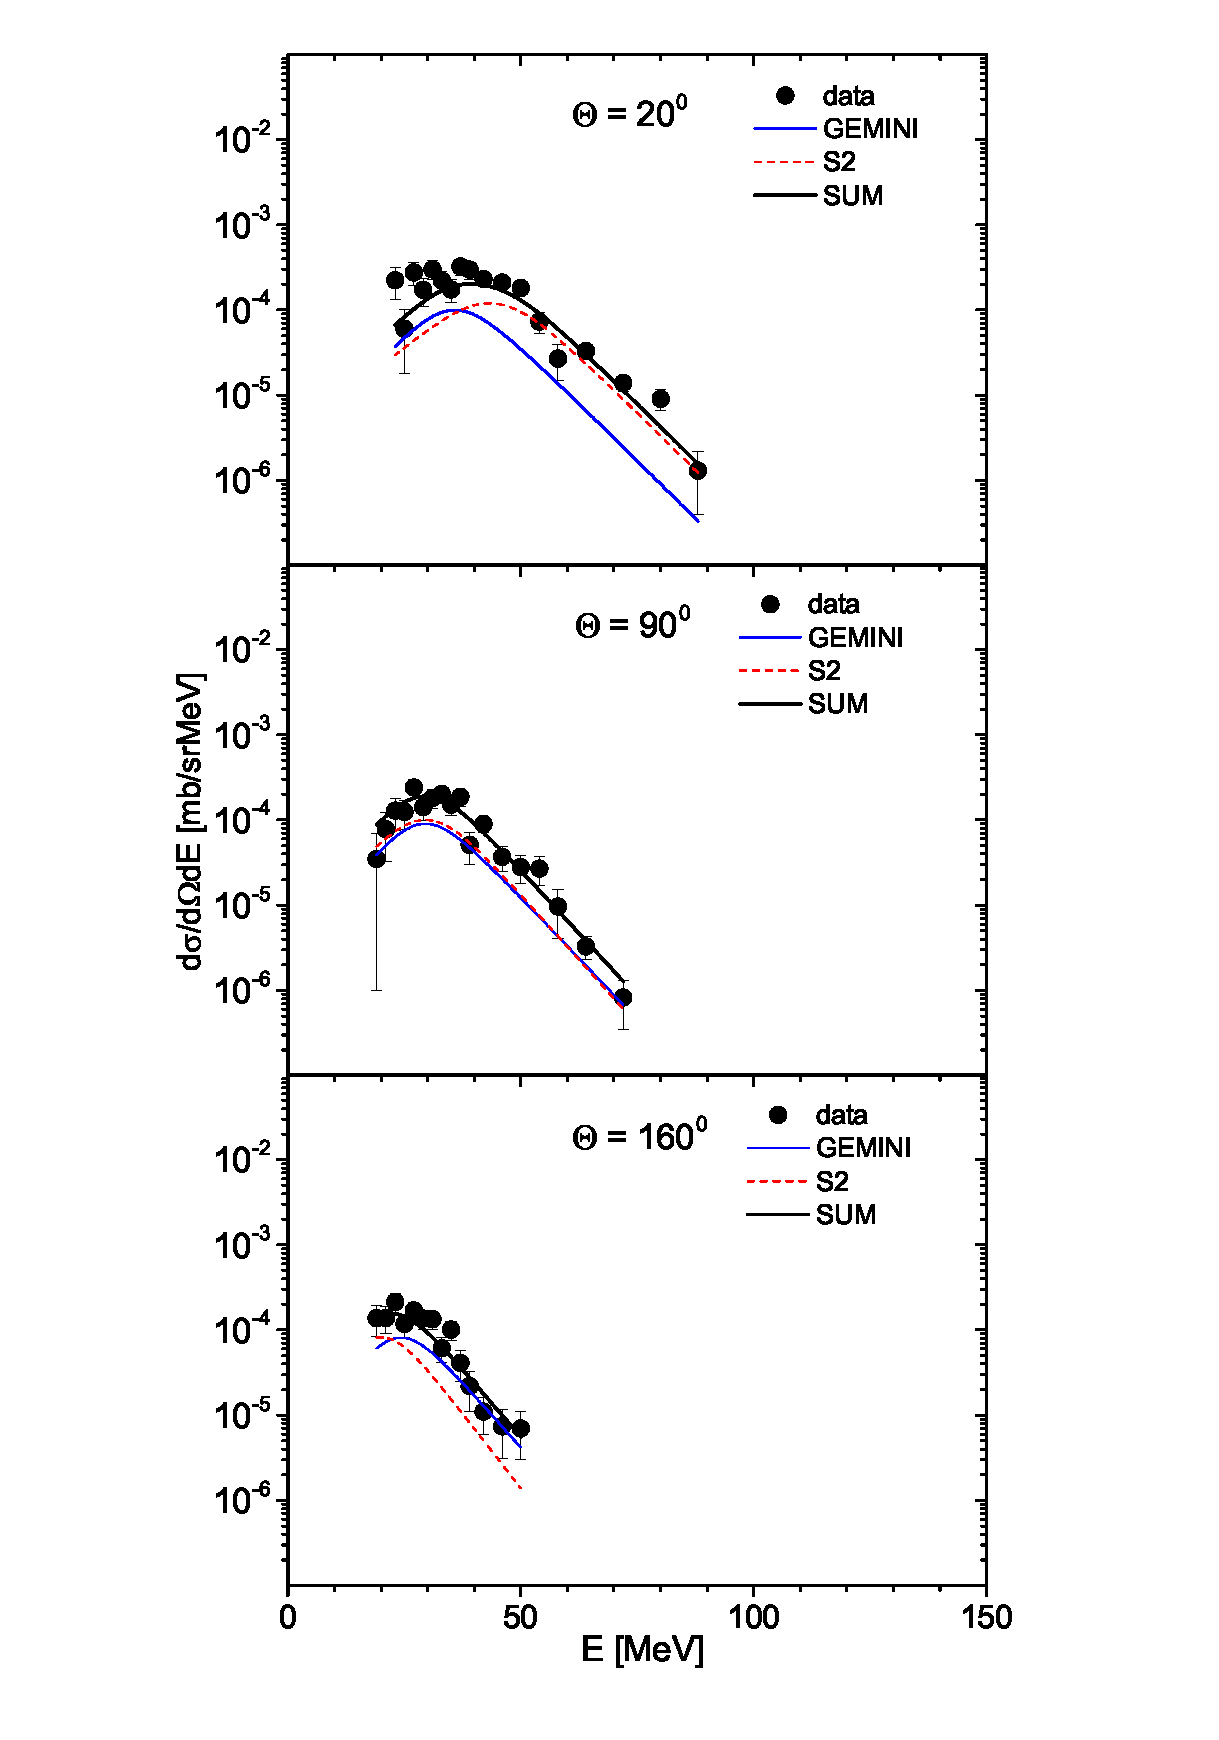
\includegraphics{18OGEMINIS2.eps}
}\\
  \caption{Experimental data (dots) and theoretical spectra for Ag(p,$^{18}$O) at three
  scattering angles: 20 degree (top panel), 90 degree (middle panel) and 120 degree (lower panel).
  The blue (solid) line represents GEMINI++ spectra, the red (dashed) line depicts contribution
  from additional moving source (S2), whereas the black (thick solid) line shows sum of both contributions.}
  \label{fig:18OGEMINIS2}
\end{figure}
%\end{figure*}
%

The procedure described above enabled us to obtain non-equilibrium
production cross section of IMF equal to the parameter $\sigma_2$ of
the slow moving source (or to the sum of $\sigma_2$ and $\sigma_3$ -
the appropriate parameters of both moving sources).  Furthermore,
sum of the equilibrium production cross section evaluated by means
of GEMINI++ and the above non-equilibrium cross section provided
value of the total production cross section.

The total cross sections due to INCL++ \cite{Mancusi2014} coupled to
GEMINI++ \cite{GEMINI++} as well as the total cross sections
obtained by fit of moving sources are presented together in Fig.
\ref{fig:SGS2S3} as a function of the atomic mass number of
ejectiles. In the lower panel of the figure the equilibrium emission
cross sections $\sigma_{\text{GEMINI}}$ are shown, in the middle
panel the non-equilibrium cross sections parameterized by slower of
the moving sources $\sigma_2$ are depicted, whereas that due to the
faster moving source $\sigma_{3}$ are shown in the upper panel of
the figure.  The cross sections for individual elements are
presented by the same symbols and are connected by lines.





%\begin{figure*}
\begin{figure}
  % Requires \usepackage{graphicx}
  \centering
  \resizebox{0.5\textwidth}{!}{%
  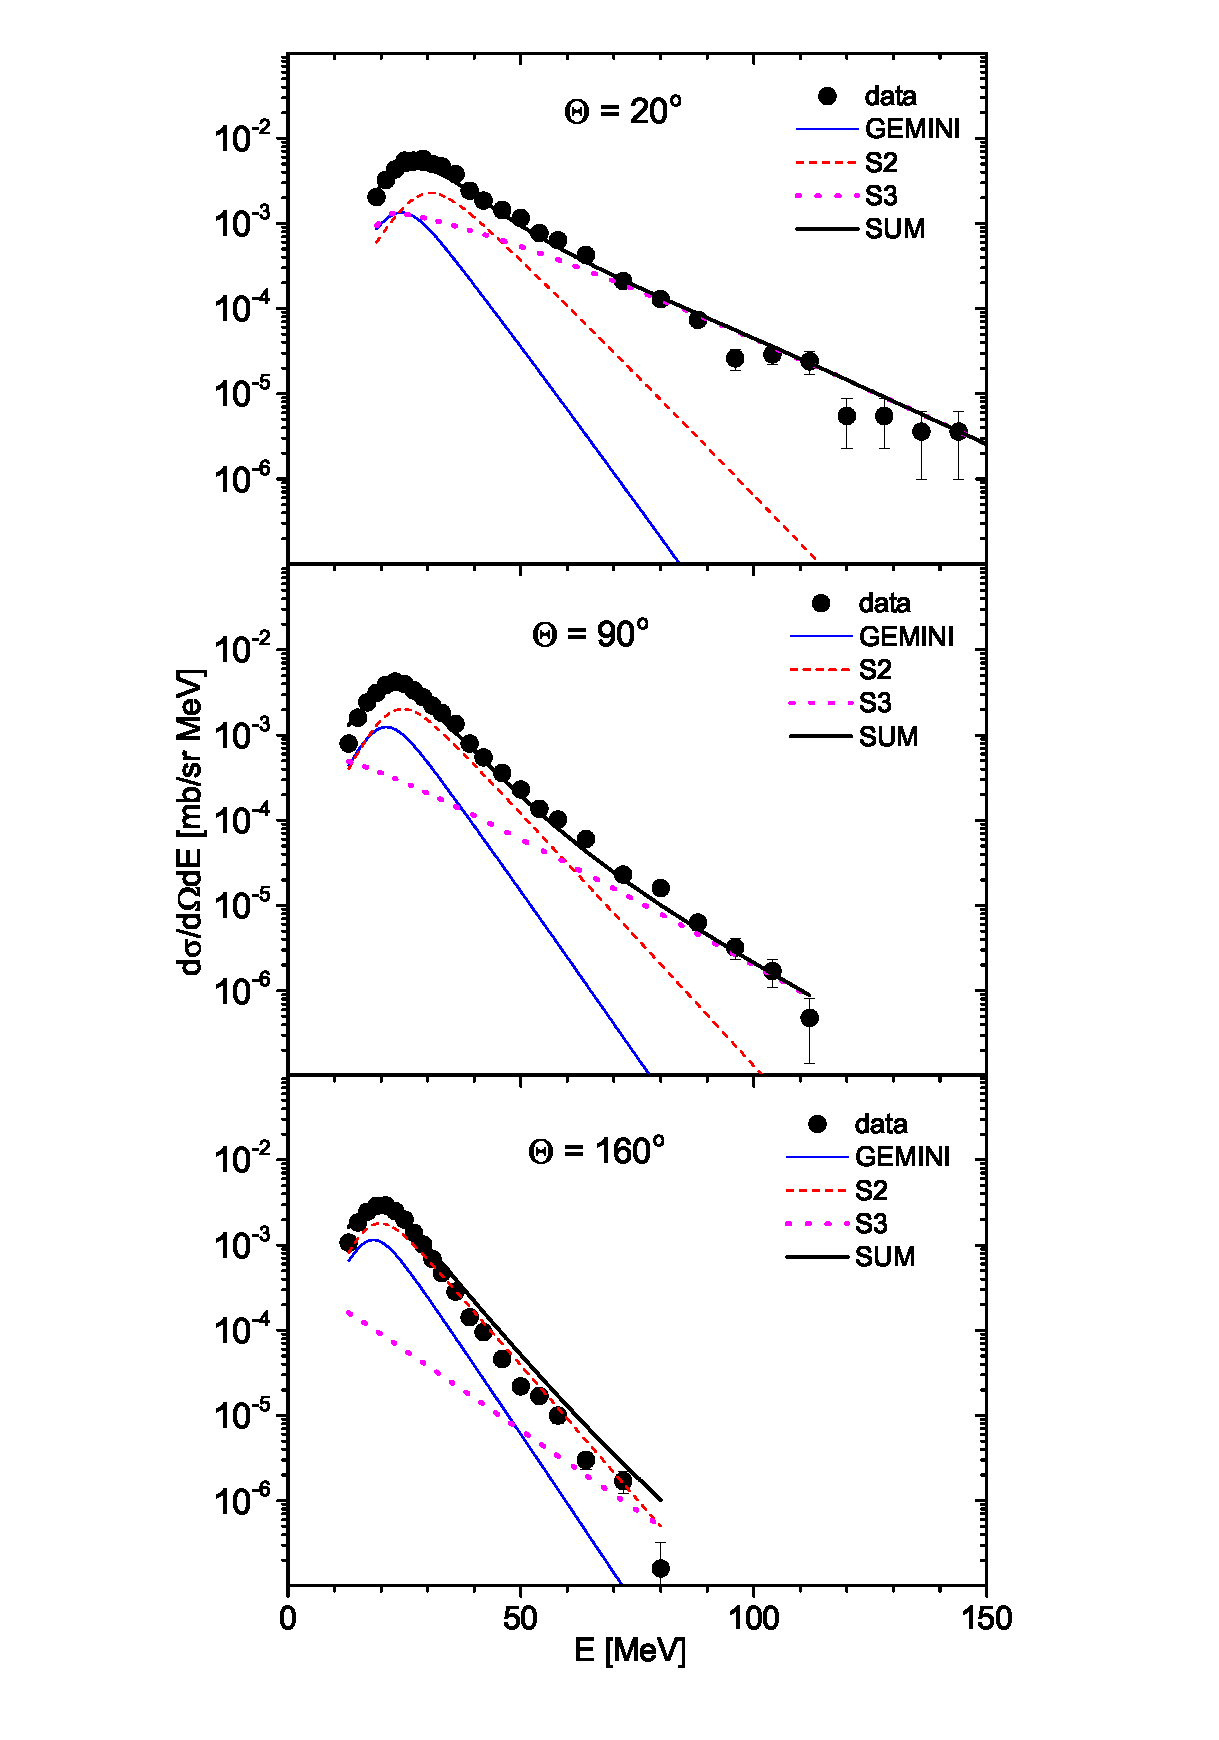
\includegraphics{9BeGEMINIS2S3.eps}
}\\
  \caption{Experimental data (dots) and theoretical spectra for Ag(p,$^9$Be) at three
  scattering angles: 20 degree (top panel), 90 degree (middle panel) and 120 degree (lower panel).
  The blue (solid) line represents GEMINI++ spectra, the red (dashed) line depicts contribution
  from slower moving source (S2), the magenta (dotted) line shows contribution of the second, faster
  source (S3) whereas the black (thick solid) line shows sum of all contributions.}
  \label{fig:9BeGEMINIS2S3}
\end{figure}
%\end{figure*}


It is clear that the cross sections decrease in average as a
function of the atomic mass number, however, this dependence of the
cross sections is non-monotonic, parabola - like  for each
individual element. It is important to note that the mass number A
of the maximal cross section  determined by the INCL+GEMINI model
for given element is not always the same as the mass number A at
which the maximal cross section of the non-equilibrium emission
appears. Furthermore, variation of the equilibrium cross sections
with the mass number seems to be more rapid than variation of the
corresponding non-equilibrium cross sections. Therefore it is quite
difficult to predict from this figure how complicated may be the
mass dependence of the ratio of non-equilibrium cross sections to
the total production cross sections
$\sigma_{\text{NEQ}}/\sigma_{\text{TOT}}$, \emph{i.e.}, to the sum
of the equilibrium and non-equilibrium cross sections.



%\begin{figure*}[H]
\begin{figure}
  % Requires \usepackage{graphicx}
  \centering
  \resizebox{0.5\textwidth}{!}{%
  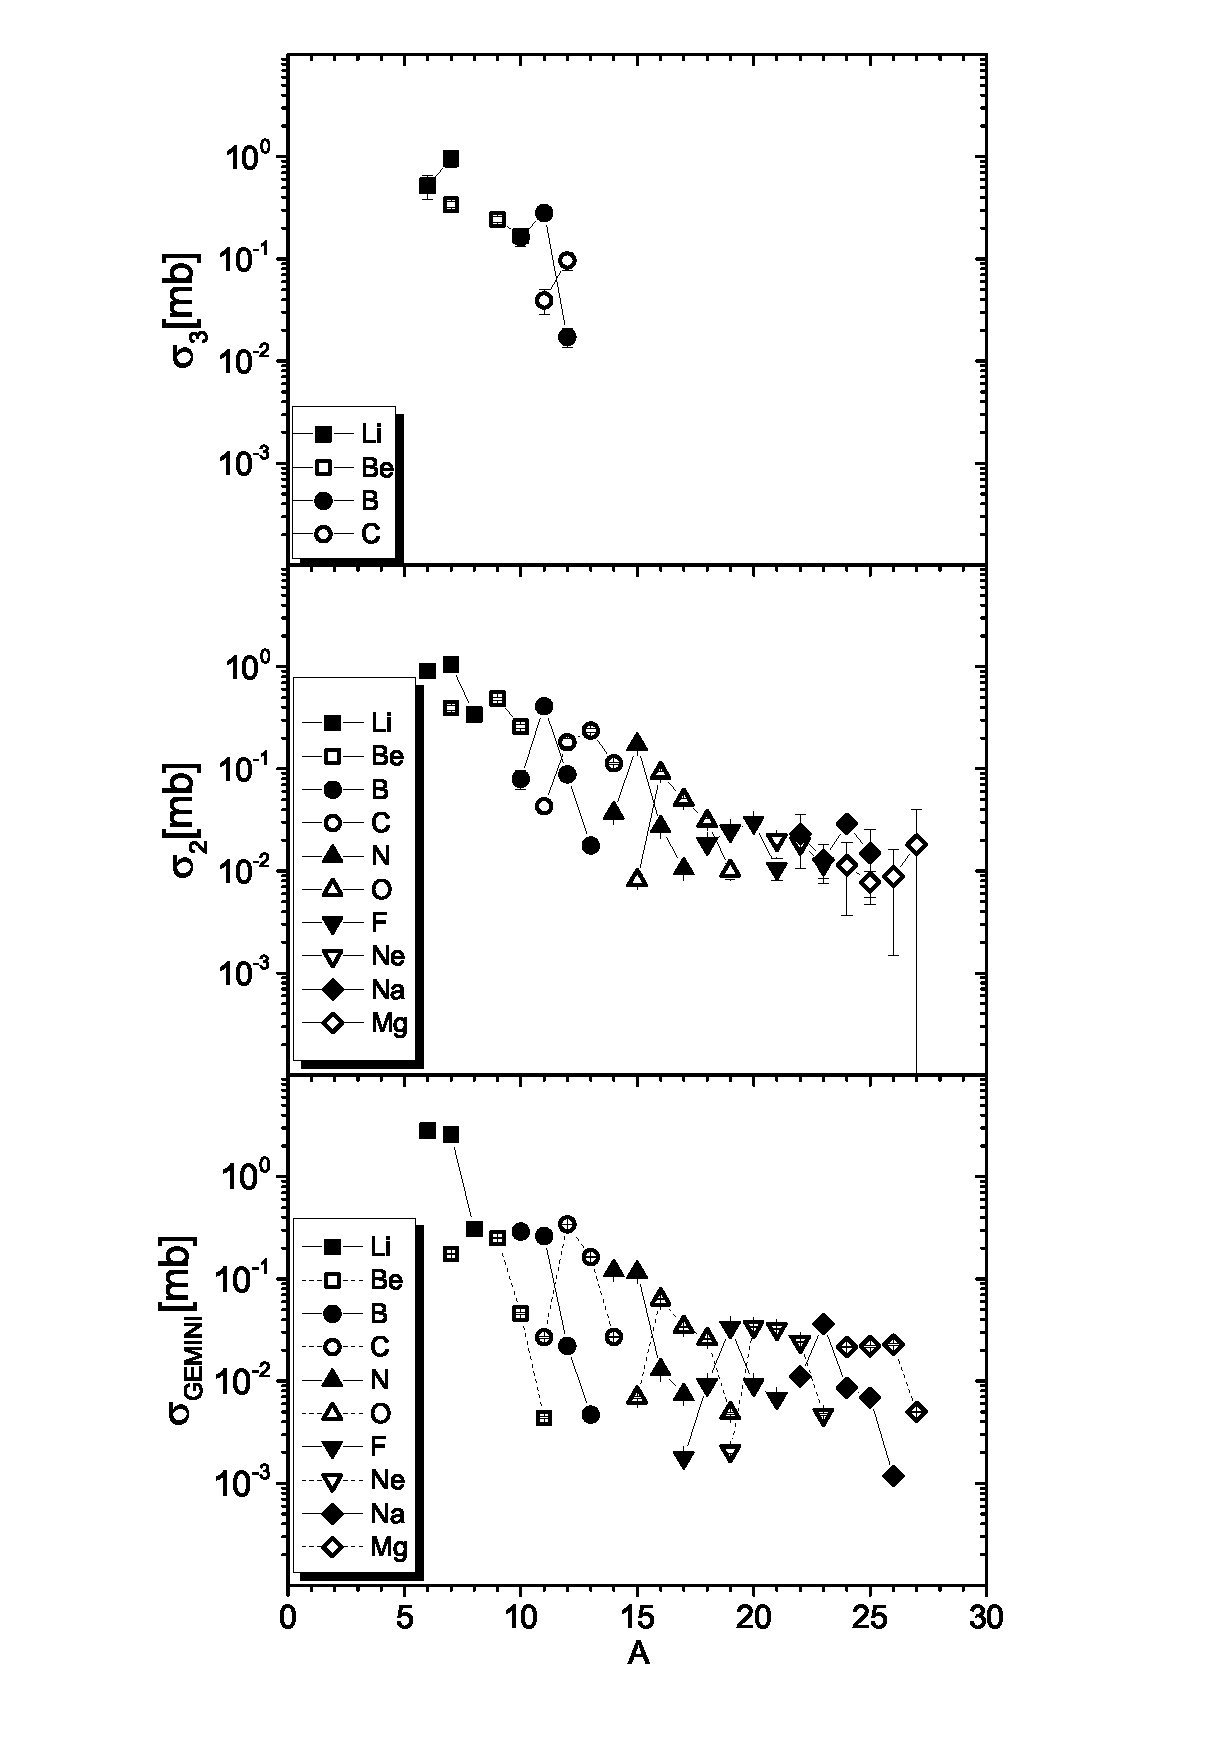
\includegraphics{SGS2S3.eps}
}\\
  \caption{Production cross sections of intermediate mass fragments evaluated by means of
  the INCL++ model coupled to the GEMINI++ one (lower panel),
  production cross sections $\sigma_2$ from the phenomenological slow moving source (middle panel) and those
  ($\sigma_3$) due to the fast moving source (upper panel).  Different elements are distinguished
  by using different symbols whereas  various isotopes
  of the same element are represented by the same symbol.}
  \label{fig:SGS2S3}
\end{figure}
%\end{figure*}
%
This quantity, which constitutes the subject of the present study is
presented in Fig. \ref{fig:RNEQtoTOTtot.eps} as a function of atomic
mass number A of produced IMF. Different symbols connected by thin
lines indicate values of the ratio for corresponding elements shown
in the description at the right hand side of the figure. The same
symbol depicts  results obtained for various isotopes of a given
element. The horizontal line placed at 0.5 value of the ratio
divides  the set of all isotopes into two groups; one with  the
ratio corresponding to the dominance of the equilibrium processes
and the second of the opposite property.



%
%
\begin{figure*}
%\begin{figure}[H]
  % Requires \usepackage{graphicx}
  \centering
  \resizebox{0.85\textwidth}{!}{%
  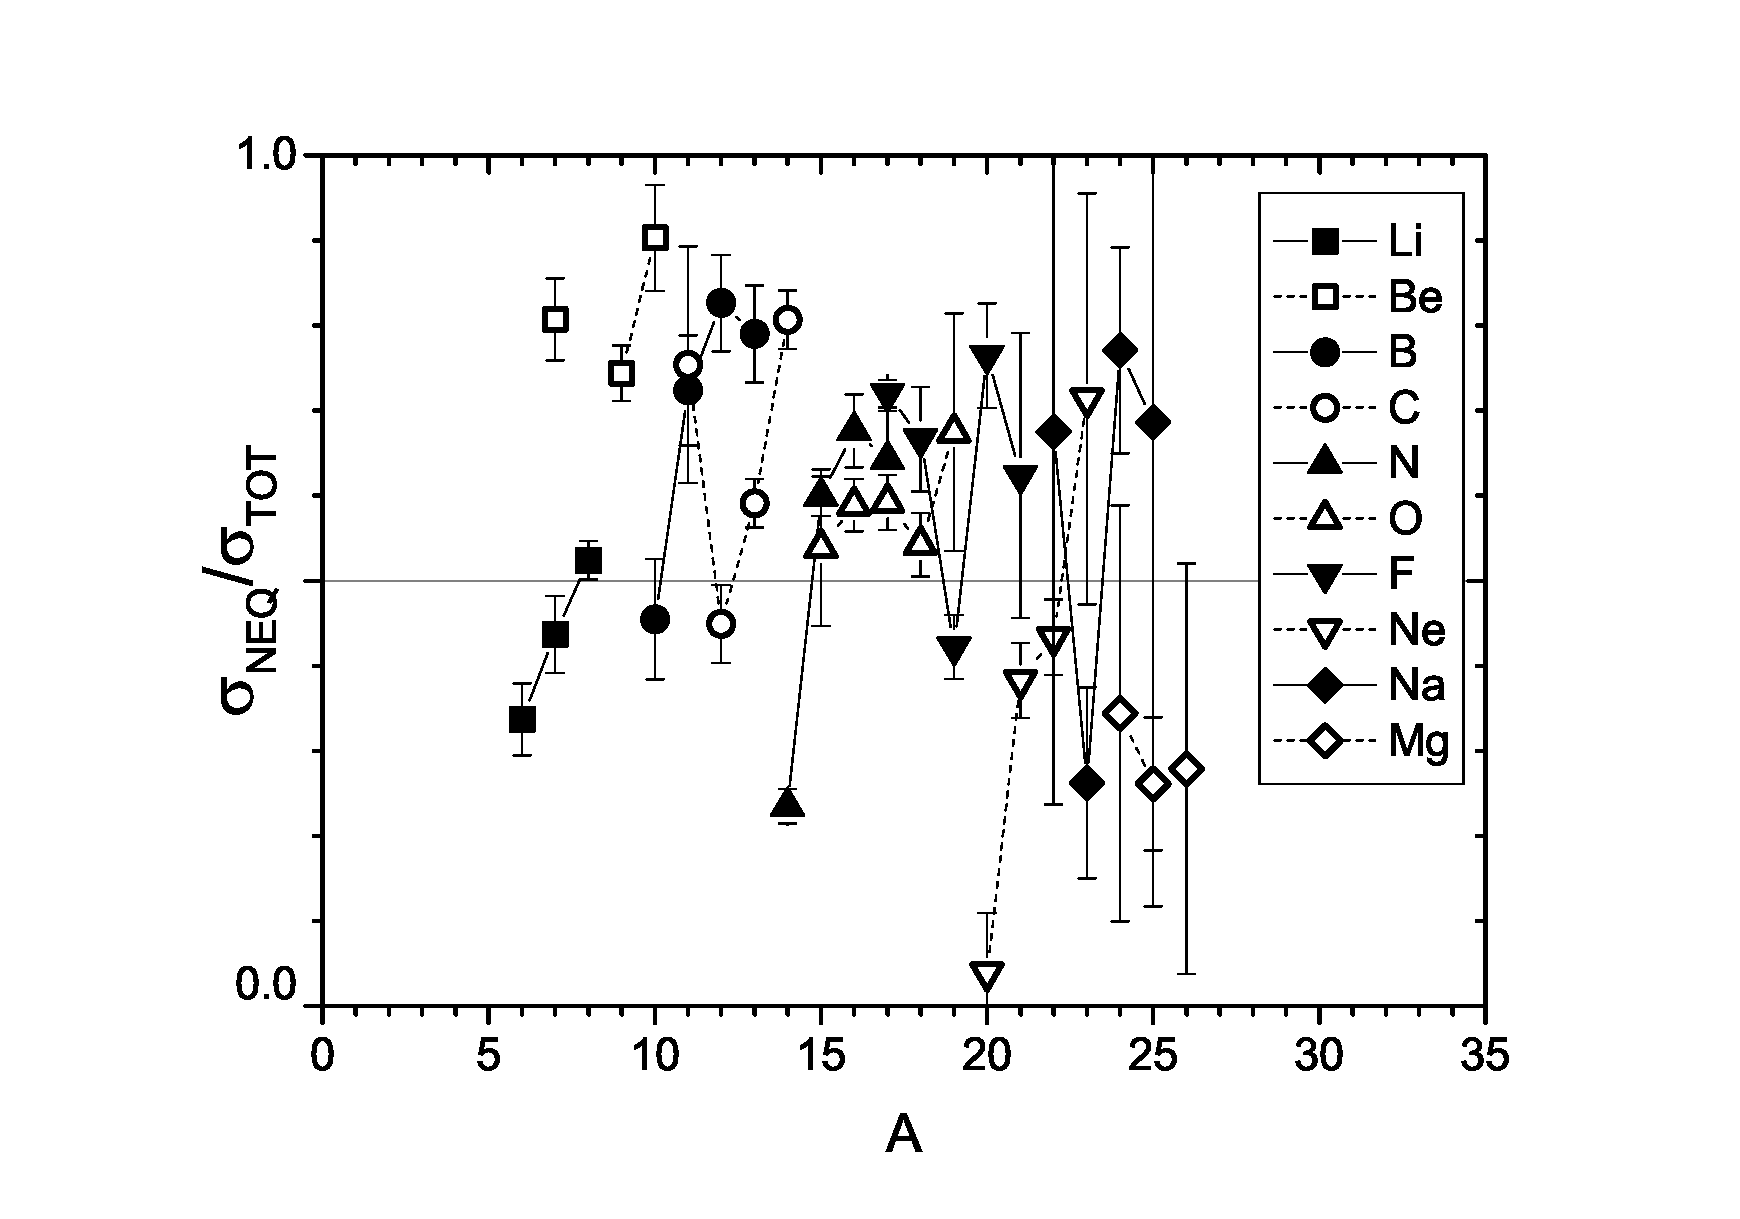
\includegraphics{RNEQtoTOTtot.eps}
}\\
  \caption{Atomic mass number A dependence of the ratio of non-equilibrium production
  cross section  to the total production cross section for intermediate mass fragments
  emerging from p+Ag collisions.
  }
  \label{fig:RNEQtoTOTtot.eps}
%\end{figure}
\end{figure*}
%





%
The following properties of the ratio of the non-equilib\-rium cross
 sections to the total cross sections may be easily
 derived from
 this figure: (i) The ratios larger than 0.5 are about 2 times more abundant
 than those smaller than 0.5.  This is true for both, small and large values
 of the atomic mass number A.
%
(ii) Values of  ratios close to 0.5 appear mainly at average
 mass number values (A $\sim$ 17) whereas those at smaller as well
 as at larger mass numbers are grouped into two separate sets.
 One set of the isotopes with the ratios smaller than 0.5
 and the second set with the ratios larger than 0.5 for the same A values.

Such a specific dependence of the ratio
$\sigma_{\text{NEQ}}/\sigma_{\text{TOT}}$ indicates that there
exists no single monotonic trend of this ratio versus mass number A
for all studied isotopes. One has to find some additional criterion
which might select the isotopes into groups behaving in the same way
when treated as a function of the mass number.

   Two specific properties of the emitted intermediate mass fragments were applied
for this purpose:

(i) the even/odd number of protons and neutrons - constituents of
the IMF, and

(ii) the third component of the isospin of the fragment T$_3 \equiv
(N-Z)/2$ representing excess (deficiency) of the number of neutrons
in respect to the number of protons. For this purpose all reaction
products were divided into 4 subgroups of definite (Z,N): (even -
even), (even - odd), (odd - even) and (odd - odd). The atomic mass
dependence of the ratio $\sigma_{\text{NEQ}}/\sigma_{\text{TOT}}$
was presented for these subgroups in separate panels of the Fig.
\ref{fig:R4eoT3}; the upper-left panel for even-even (Z,N), the
upper-right one for even-odd, \emph{etc.}, in the clockwise
direction.

It turned out that the ratio
$\sigma_{\text{NEQ}}/\sigma_{\text{TOT}}$ behaves in a very regular
way for each of these selected groups of isotopes (cf. Fig.
\ref{fig:R4eoT3}). Especially, it may be stated that this ratio
decreases in average linearly with the mass number A of emitted
fragment for even-even, even-odd and odd-even intermediate mass
fragments whereas it increases in average linearly for odd-odd
ejectiles.

Furthermore, some deviations from such a regular behaviour may be
observed for specific values of the third component of the isospin
$T_3 \equiv (N-Z)/2$ of the emitted particles. For example, two of
the four even-even ejectiles with $T_3=0$, namely $^{12}$C and
$^{20}$Ne have much smaller ratio
$\sigma_{\text{NEQ}}/\sigma_{\text{TOT}}$ than other even-even IMF
with $T_3=0$ and all $T_3=1$ particles %which very well follow a
%straight, decreasing line versus the atomic mass number A
(cf.
upper, left panel of Fig. \ref{fig:R4eoT3}).

 Second of such
deviations is the fact that all $T_3=3/2$ nuclides for even-odd and
odd-even ejectiles have larger
$\sigma_{\text{NEQ}}/\sigma_{\text{TOT}}$ ratio than that which
characterizes the $T_3=-1/2$ and $T_3=1/2$ nuclides (cf. upper-right
and lower-right panel of the Fig. \ref{fig:R4eoT3}).

The third example consists in the systematic deviation toward
smaller ratio values of $T_3=0$ ejectiles in respect to the straight
line averaging behaviour of the odd-odd group of ejectiles whereas
the IMF with $T_3=1$ deviate toward larger ratio values (cf.
lower-left panel of the Fig. \ref{fig:R4eoT3}).



\begin{figure*}
%\begin{figure}[H]
  % Requires \usepackage{graphicx}
  \centering
  \resizebox{0.85\textwidth}{!}{%
  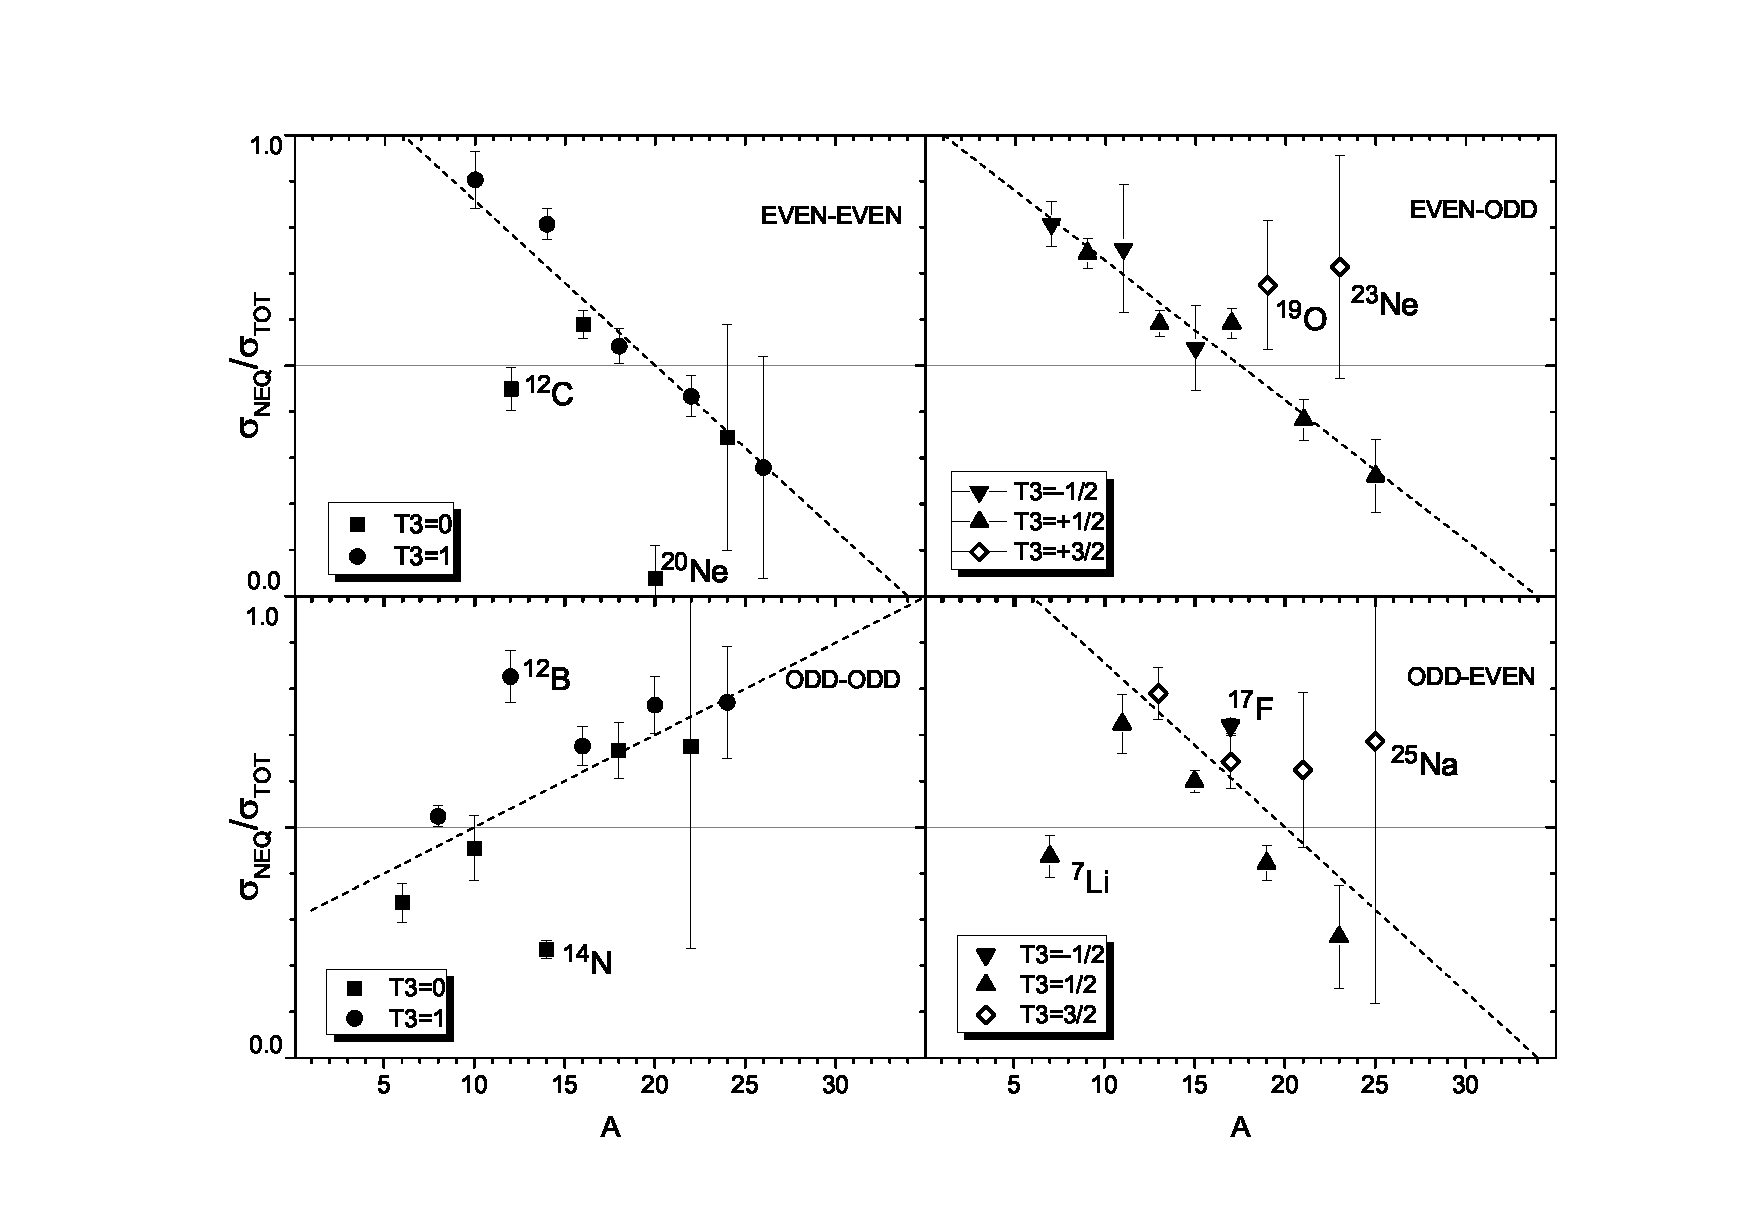
\includegraphics{R4eoT3.eps}
}\\
  \caption{Atomic mass number A dependence of the ratio of non-equilibrium production
  cross section to the total production cross section for intermediate mass fragments
  emerging from p+Ag collisions.  % at proton beam energy E$_p$=0.48 GeV.
  Left upper panel of the figure presents the results for even-even (Z,N) products
  whereas other panels
  (in clockwise direction) contain results for even-odd, odd-even and odd-odd products.
  Different symbols are attributed to values of the ratio corresponding to different values of the third
  component of the isospin $T_3=(N-Z)/A$ of ejectiles. Dashed lines are drawn to guide the eye.}
  \label{fig:R4eoT3}
%\end{figure}
\end{figure*}


While no physical model has been implied by the dependence presented
in the Fig. \ref{fig:R4eoT3}, the extremely regular behaviour
achieved in this  analysis certainly merits further consideration.




%
%
\begin{figure*}
%%\begin{figure}[H]
  % Requires \usepackage{graphicx}
  \centering
  \resizebox{0.8\textwidth}{!}{%
  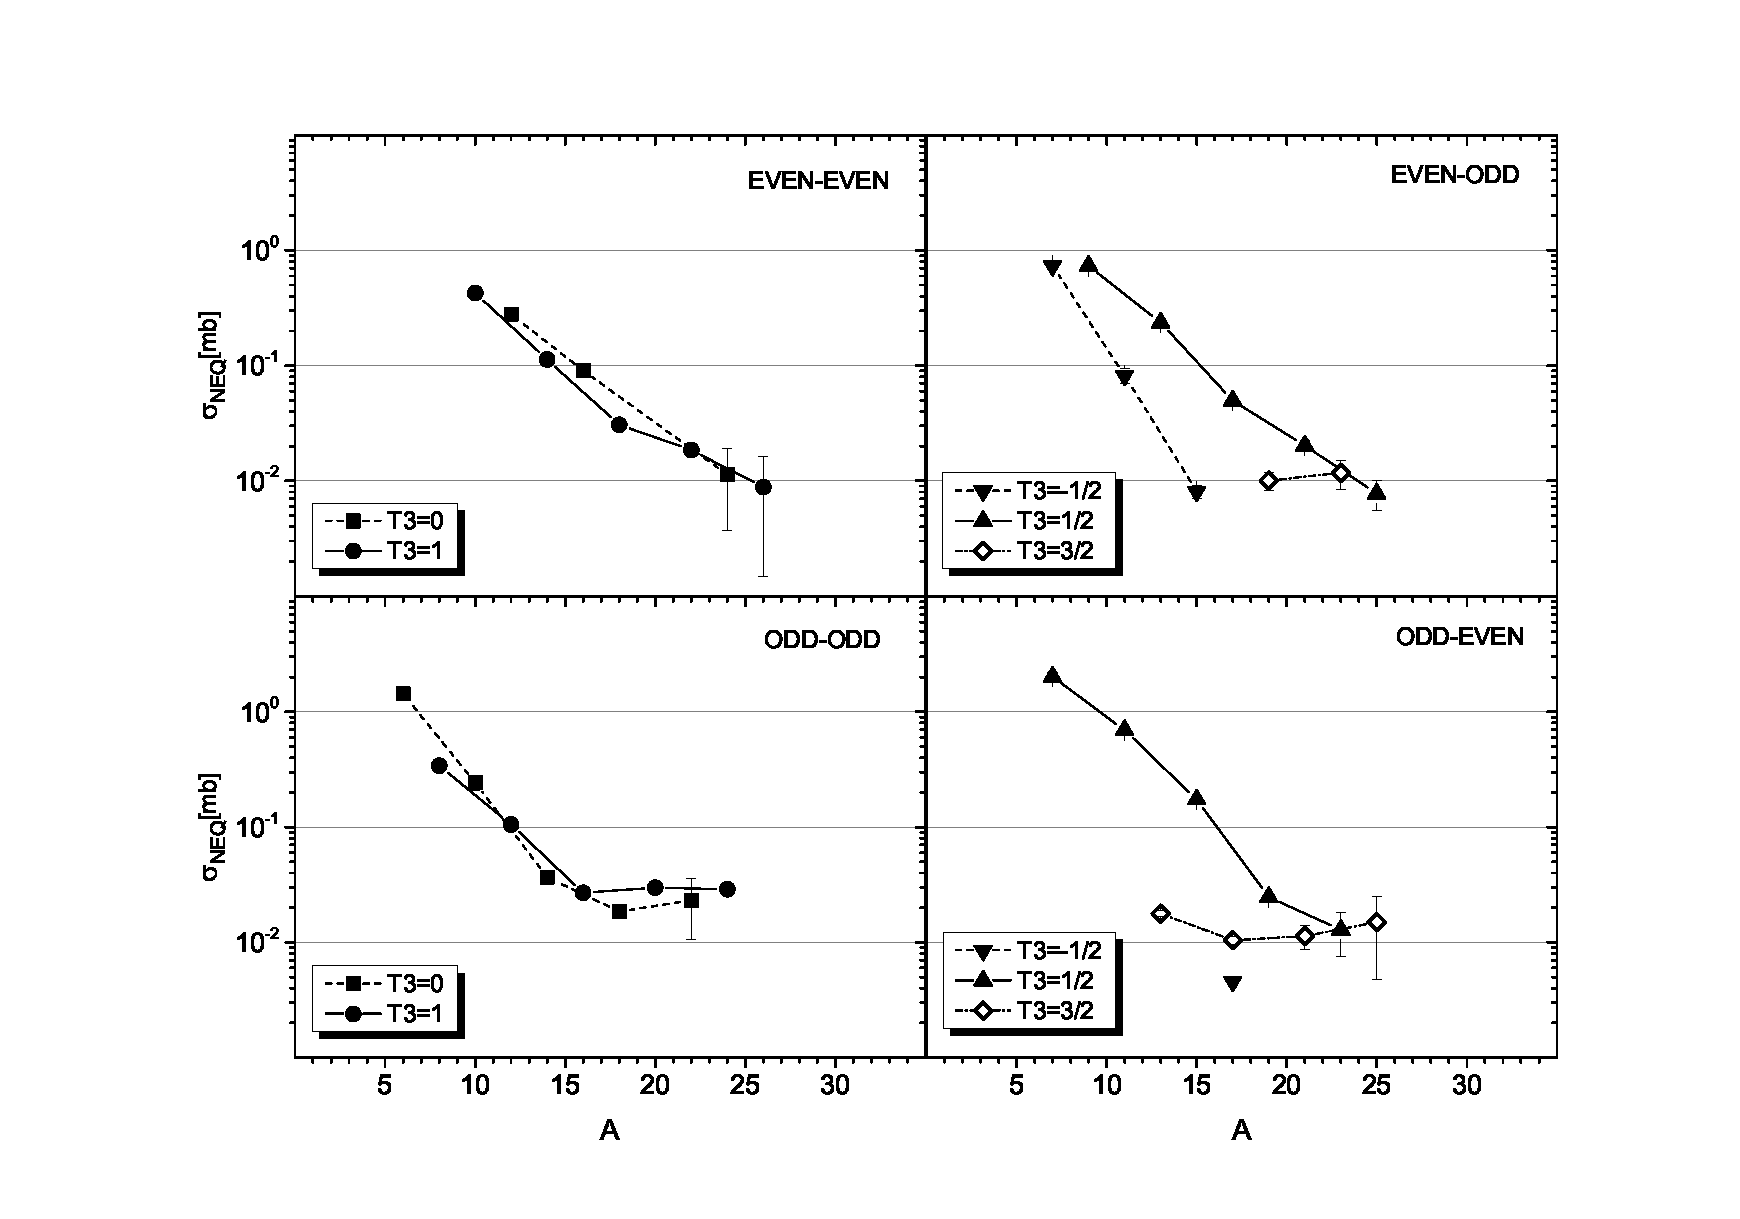
\includegraphics{S23vsAT3.eps}
}\\
  \caption{Atomic mass number dependence of  the production
  cross sections of intermediate mass fragments
  emerging due to non-equilibrium processes from p+Ag collisions.   Left upper panel
  of the figure presents the results for even-even (Z,N) products whereas other panels
  (in clockwise direction) contain results for even-odd, odd-even and odd-odd products.
  Different symbols are attributed to values of the cross sections for fragments with different values of the third
  component of the isospin $T_3=(N-Z)/A$. The solid, dashed and dot-dashed lines are drawn to guide the eye.}
  \label{fig:S23vsAT3}
%%\end{figure}
\end{figure*}


\begin{figure*}
%%\begin{figure}[H]
  % Requires \usepackage{graphicx}
  \centering
  \resizebox{0.8\textwidth}{!}{%
  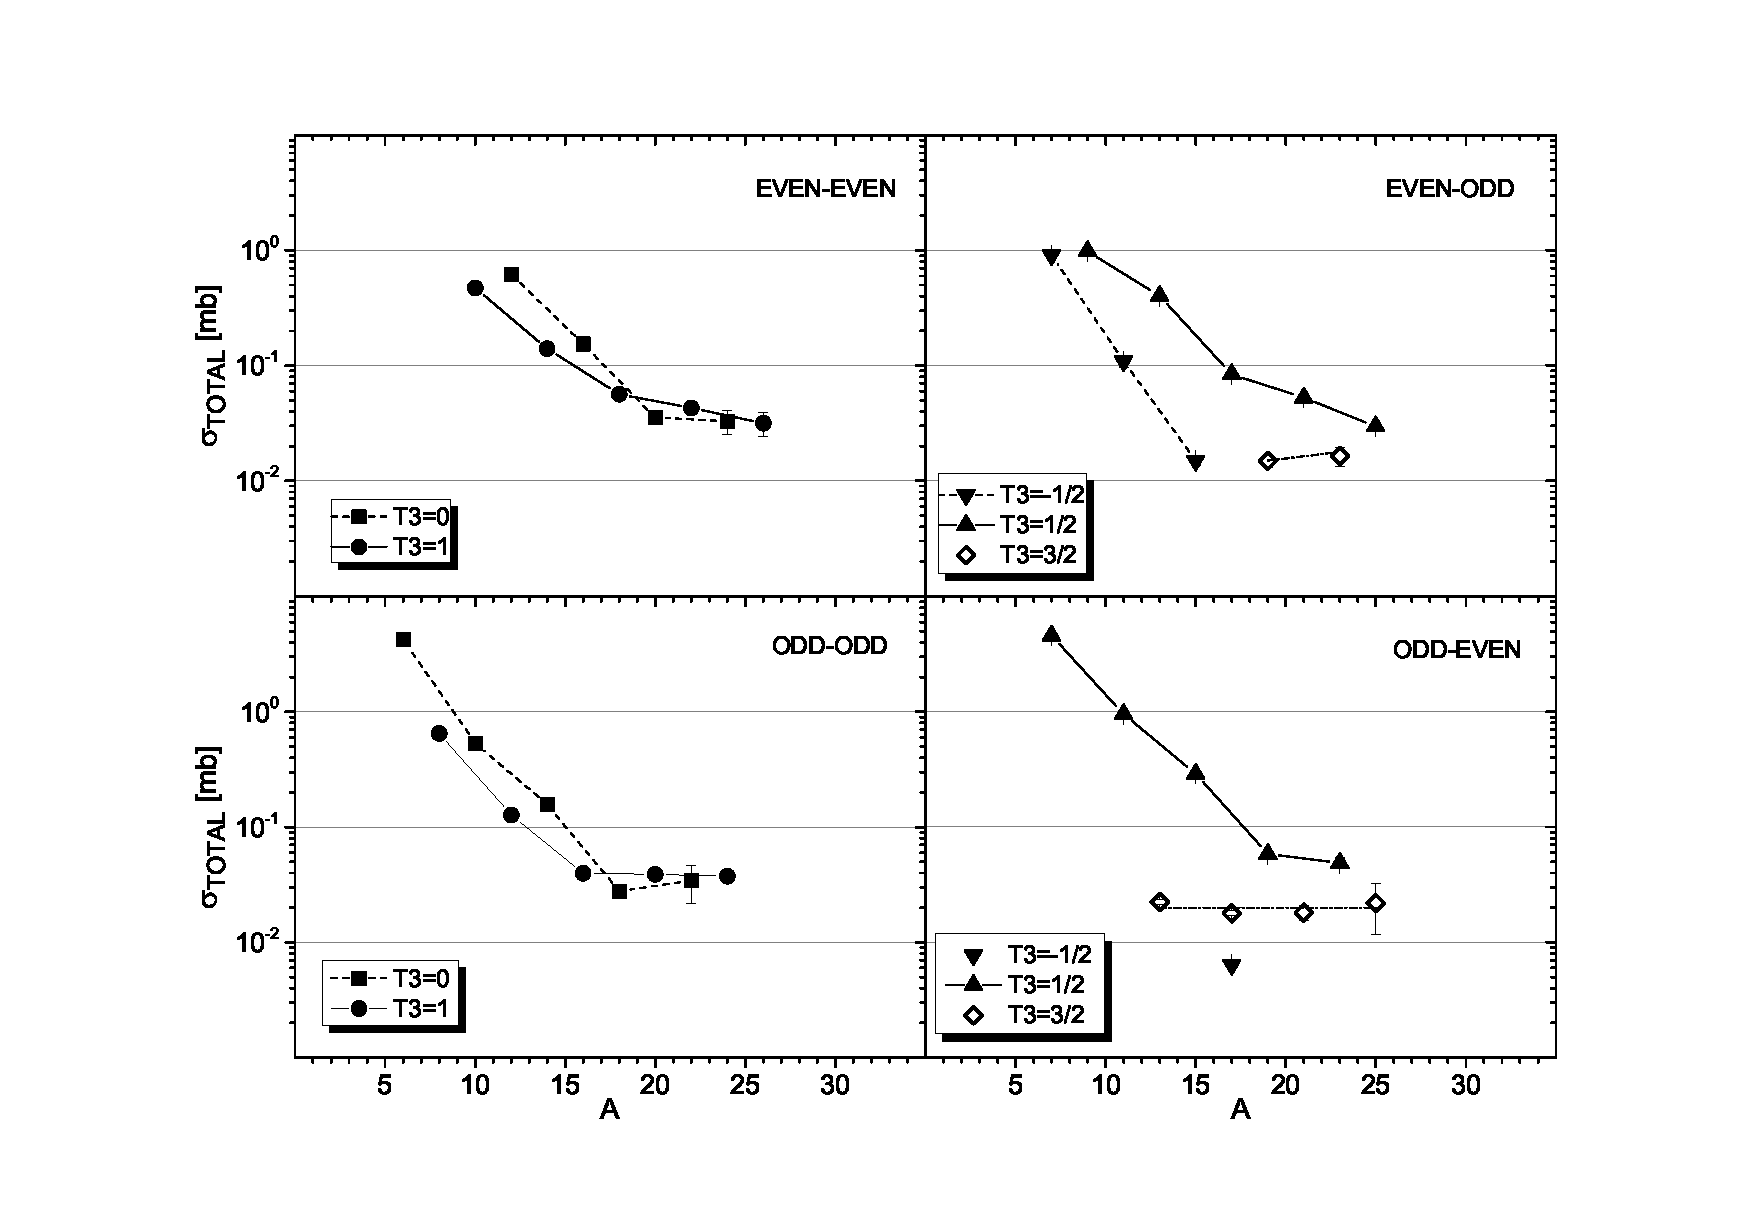
\includegraphics{TOTG23T3.eps}
}\\
  \caption{The same as in Fig. \ref{fig:S23vsAT3} but for the total
  production cross sections, \emph{i.e.}, for the sum of equilibrium and non-equilibrium production cross sections.
  The solid, dashed and dot-dashed lines are drawn to guide the eye.
%  Atomic mass dependence of  the equilibrium production
%  cross section evaluated by GEMINI++ for intermediate mass fragments
%  emerging from p+Ag collisions at proton beam energy E$_p$=0.48 GeV. Left upper panel
%  of the figure presents the results for even-even (Z,N) products whereas other panels
%  (in clockwise direction) contain results for even-odd, odd-even and odd-odd products.
%  Different symbols are attributed to values of the cross sections for fragments with different values of the third
%  component of the isospin $T_3=(N-Z)/A$. The solid, dashed and dot-dashed lines are drawn to guide the eye.
  }
  \label{fig:TOTG23T3}
%%\end{figure}
\end{figure*}





\begin{figure*}
%%\begin{figure}[H]
  % Requires \usepackage{graphicx}
  \centering
  \resizebox{0.8\textwidth}{!}{%
  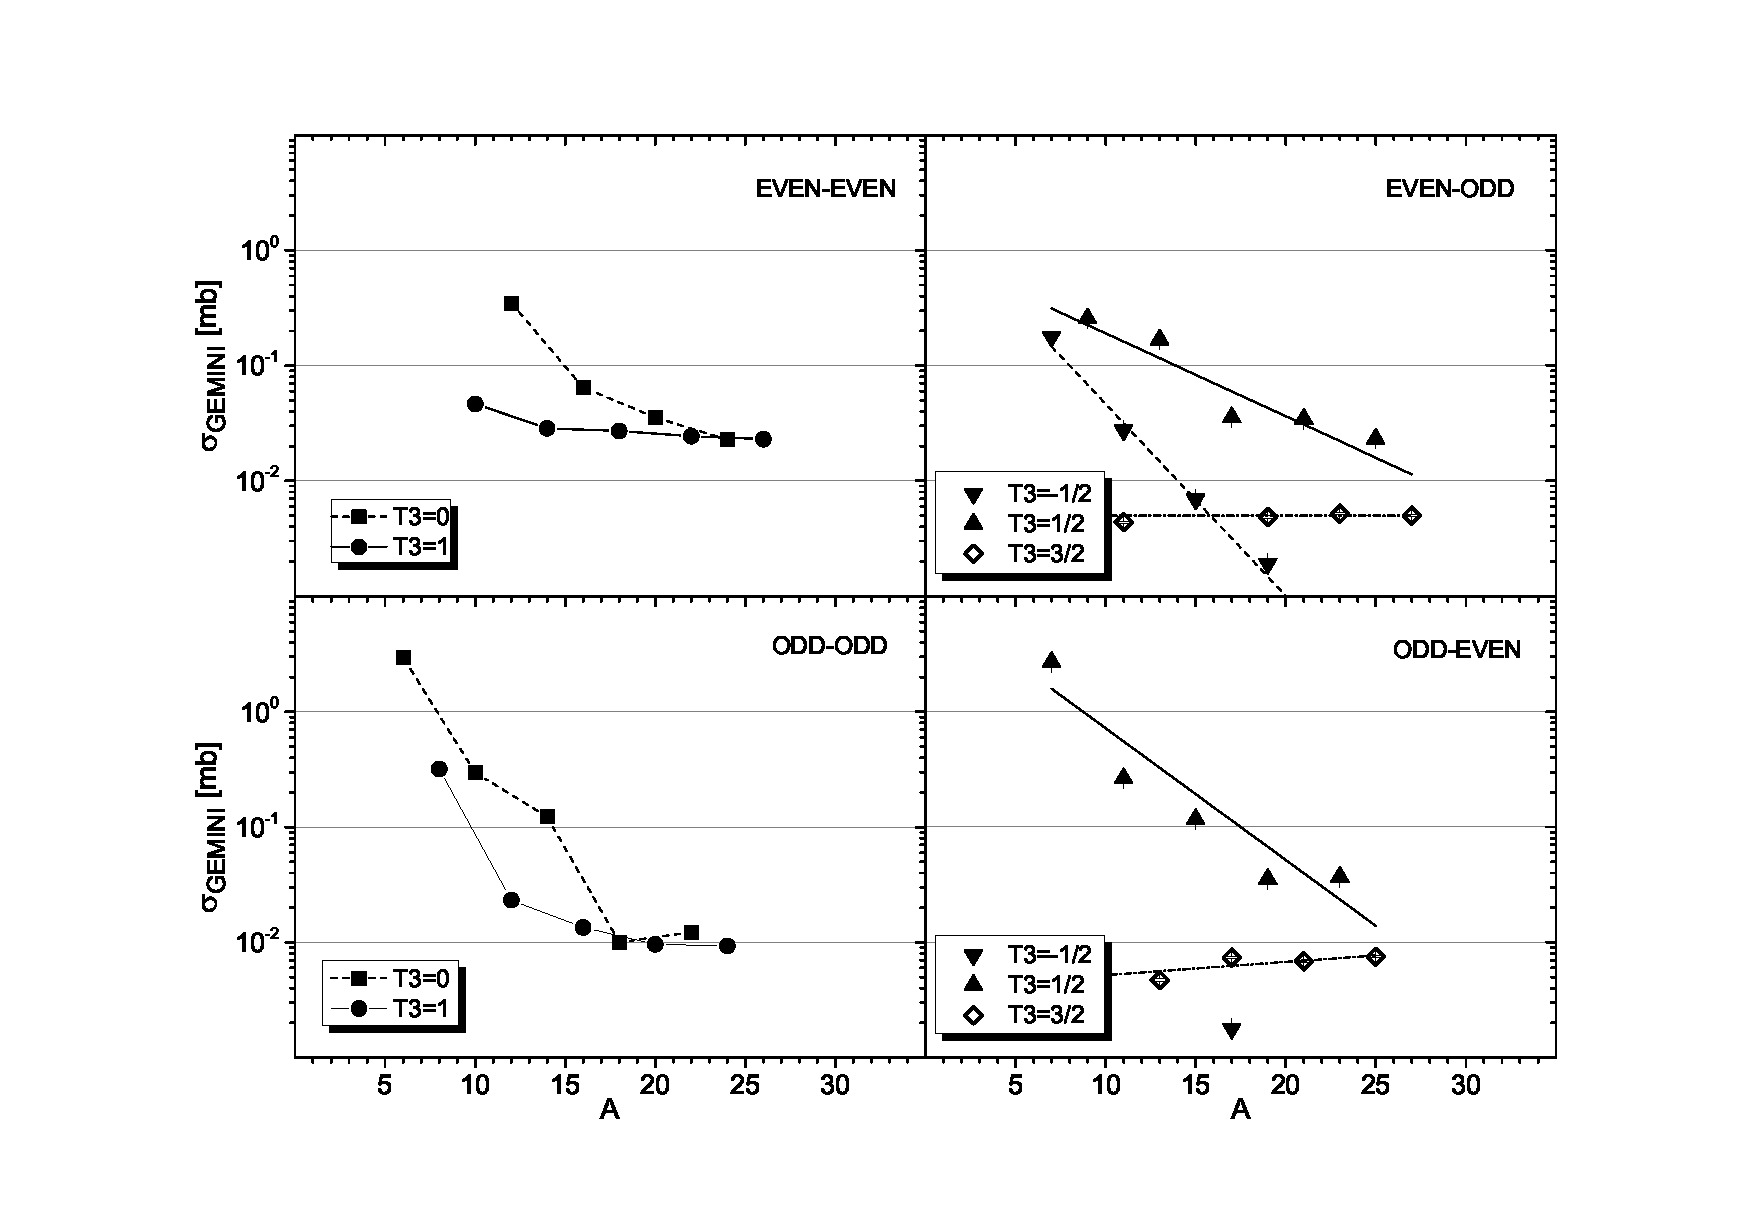
\includegraphics{GEMseparateT3.eps}
}\\
  \caption{The same as in Fig. \ref{fig:S23vsAT3} but for the equilibrium
  emission cross sections evaluated by means of the INCL++ plus GEMINI++
  models. The solid, dashed and dot-dashed lines are drawn to guide the eye.
%  Atomic mass dependence of  the equilibrium production
%  cross section evaluated by GEMINI++ for intermediate mass fragments
%  emerging from p+Ag collisions at proton beam energy E$_p$=0.48 GeV. Left upper panel
%  of the figure presents the results for even-even (Z,N) products whereas other panels
%  (in clockwise direction) contain results for even-odd, odd-even and odd-odd products.
%  Different symbols are attributed to values of the cross sections for fragments with different values of the third
%  component of the isospin $T_3=(N-Z)/A$. The solid, dashed and dot-dashed lines are drawn to guide the eye.
  }
  \label{fig:GEMseparateT3}
%%\end{figure}
\end{figure*}
 %
\section{Hybrid (phenomenological+microscopic) approach to describe the double-differential cross sections features of total cross sections – odd-even staggering}
\section{Comparison of models and conclusion about their limitation}